\newif\ifshowsolutions
\showsolutionstrue
\documentclass{article}
\usepackage{listings}
\usepackage{amsmath}
%\usepackage{subfigure}
\usepackage{subfig}
\usepackage{amsthm}
\usepackage{amsmath}
\usepackage{amssymb}
\usepackage{graphicx}
\usepackage{mdwlist}
\usepackage[colorlinks=true]{hyperref}
\usepackage{geometry}
\usepackage{titlesec}
\geometry{margin=1in}
\geometry{headheight=2in}
\geometry{top=2in}
\usepackage{palatino}
\usepackage{mathrsfs}
\usepackage{fancyhdr}
\usepackage{paralist}
\usepackage{todonotes}
\setlength{\marginparwidth}{2.15cm}
\usepackage{tikz}
\usetikzlibrary{positioning,shapes,backgrounds}
\usepackage{float} % Place figures where you ACTUALLY want it
\usepackage{comment} % a hack to toggle sections
\usepackage{ifthen}
\usepackage{mdframed}
\usepackage{verbatim}
\usepackage[strings]{underscore}
\usepackage{listings}
\usepackage{bbm}
\rhead{}
\lhead{}

\renewcommand{\baselinestretch}{1.15}

% Shortcuts for commonly used operators
\newcommand{\E}{\mathbb{E}}
\newcommand{\Var}{\operatorname{Var}}
\newcommand{\Cov}{\operatorname{Cov}}
\newcommand{\Bias}{\operatorname{Bias}}
\DeclareMathOperator{\argmin}{arg\,min}
\DeclareMathOperator{\argmax}{arg\,max}

% do not number subsection and below
\setcounter{secnumdepth}{1}

% custom format subsection
\titleformat*{\subsection}{\large\bfseries}

% set up the \question shortcut
\newcounter{question}[section]
\newenvironment{question}[1][]
  {\refstepcounter{question}\par\addvspace{1em}\textbf{Question~\Alph{question}\!
    \ifthenelse{\equal{#1}{}}{}{ [#1 points]}: }}
    {\par\vspace{\baselineskip}}

\newcounter{subquestion}[question]
\newenvironment{subquestion}[1][]
  {\refstepcounter{subquestion}\par\medskip\textbf{\roman{subquestion}.\!
    \ifthenelse{\equal{#1}{}}{}{ [#1 points]:}} }
  {\par\addvspace{\baselineskip}}

\titlespacing\section{0pt}{12pt plus 2pt minus 2pt}{0pt plus 2pt minus 2pt}
\titlespacing\subsection{0pt}{12pt plus 4pt minus 2pt}{0pt plus 2pt minus 2pt}
\titlespacing\subsubsection{0pt}{12pt plus 4pt minus 2pt}{0pt plus 2pt minus 2pt}


\newenvironment{hint}[1][]
  {\begin{em}\textbf{Hint: }}{\end{em}}

\ifshowsolutions
  \newenvironment{solution}[1][]
    {\par\medskip \begin{mdframed}\textbf{Solution~\Alph{question}#1:} \begin{em}}
    {\end{em}\medskip\end{mdframed}\medskip}
  \newenvironment{subsolution}[1][]
    {\par\medskip \begin{mdframed}\textbf{Solution~\Alph{question}#1.\roman{subquestion}:} \begin{em}}
    {\end{em}\medskip\end{mdframed}\medskip}
\else
  \excludecomment{solution}
  \excludecomment{subsolution}
\fi

\newcommand{\boldline}[1]{\underline{\textbf{#1}}}

\chead{%
  {\vbox{%
      \vspace{2mm}
      \large
      Machine Learning \& Data Mining \hfill
      Caltech CS/CNS/EE 155 \hfill \\[1pt]
      Miniproject 2 Visualizations\hfill
      Due February $23^{rd}$, 2018 \\
    }
  }
}

\begin{document}
\pagestyle{fancy}

\begin{itemize}

    \item \boldline{Group members} \\
    Mia de los Reyes, Lee Rosenthal, and Devin Cody
    
    \item \boldline{Team name} \\
    Team Segfault
    
\end{itemize}

\section{Basic Visualizations}

\subsection{All ratings in the MovieLens Dataset}
    \begin{figure}[H]
    \centering
    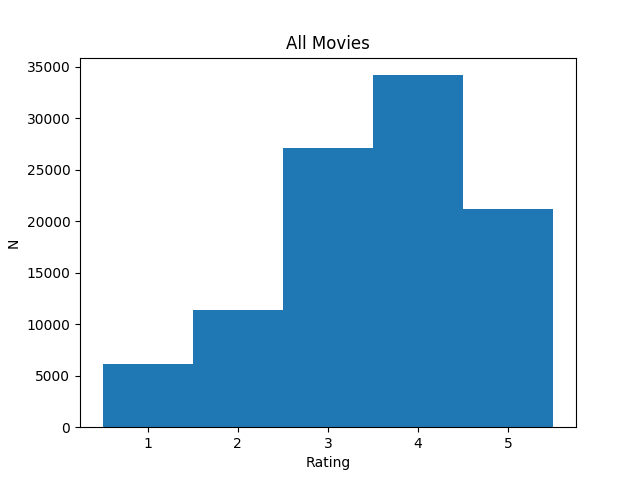
\includegraphics[width=0.75\textwidth]{../Figures/allratings.png}
    \caption{All ratings.}
    \end{figure}
    
\subsection{All ratings of the ten most popular movies}
    \begin{figure}[H]
    \centering
    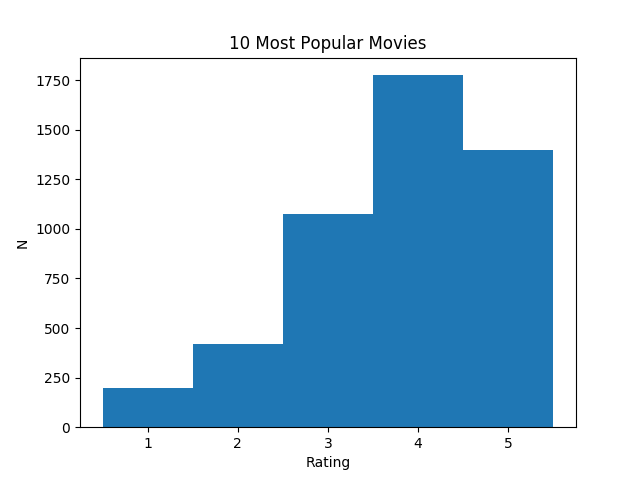
\includegraphics[width=0.6\textwidth]{../Figures/10mostpopratings.png}
    \caption{10 most popular ratings.}
    \end{figure}
    
\subsection{All ratings of the ten best movies}    
    \begin{figure}[H]
    \centering
    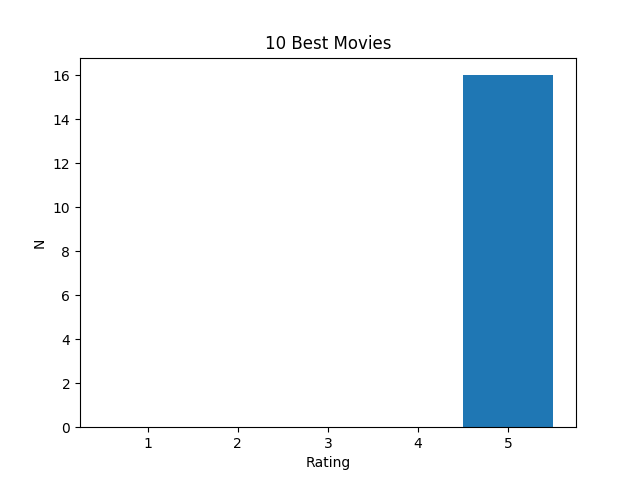
\includegraphics[width=0.6\textwidth]{../Figures/10bestratings.png}
    \caption{10 best ratings.}
    \end{figure}

\subsection{All ratings of movies from three genres}
    \begin{figure}[H]
    \centering
    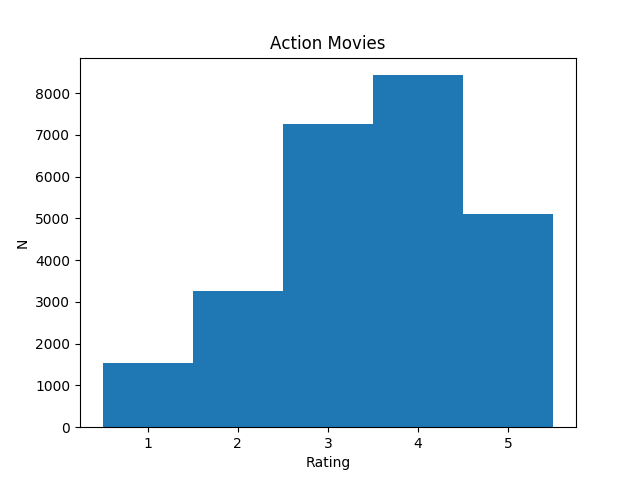
\includegraphics[width=0.6\textwidth]{../Figures/Actionratings.png}
    \caption{Action ratings.}
    \end{figure}
    \begin{figure}[H]
    \centering
    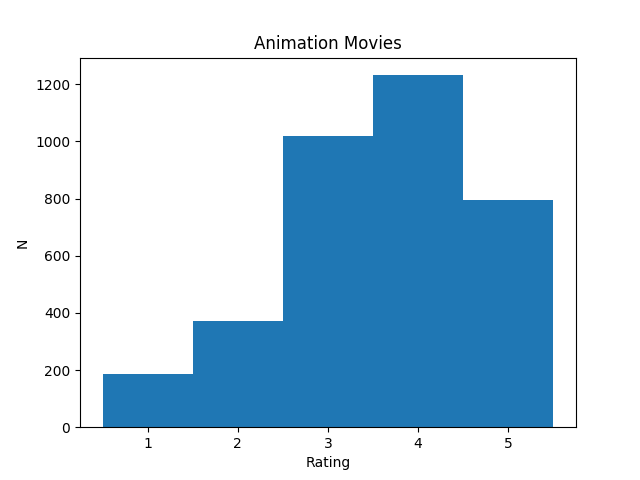
\includegraphics[width=0.6\textwidth]{../Figures/Animationratings.png}
    \caption{Animation ratings.}
    \end{figure}
    \begin{figure}[H]
    \centering
    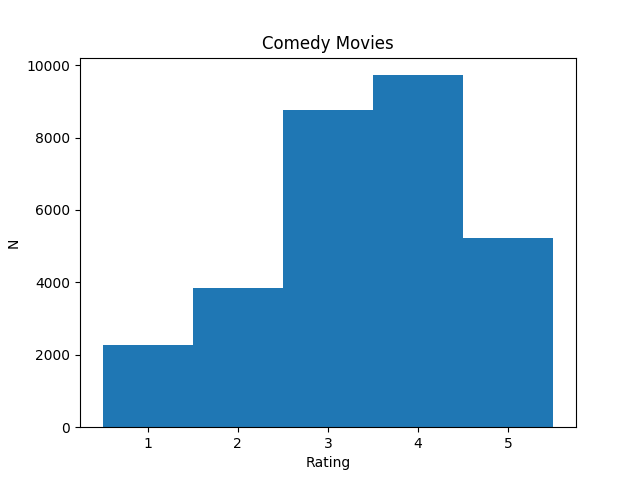
\includegraphics[width=0.6\textwidth]{../Figures/Comedyratings.png}
    \caption{Comedy ratings.}
    \end{figure}

\section{Matrix Factorization Visualizations}

\subsection{Any ten movies of your choice from the MovieLens dataset.}
    \begin{figure}[H]
    \centering
    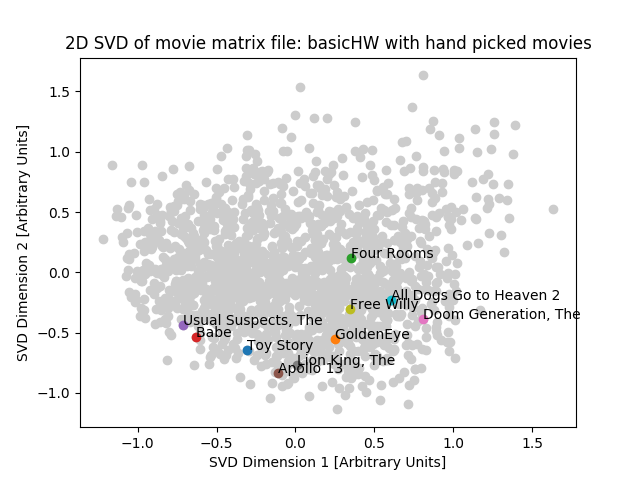
\includegraphics[width=0.75\textwidth]{../Figures/fig1.png}
    \caption{Ten handpicked movies, using basic factorization from HW5.}
    \end{figure}

\subsection{The ten most popular movies}    
    \begin{figure}[H]
    \centering
    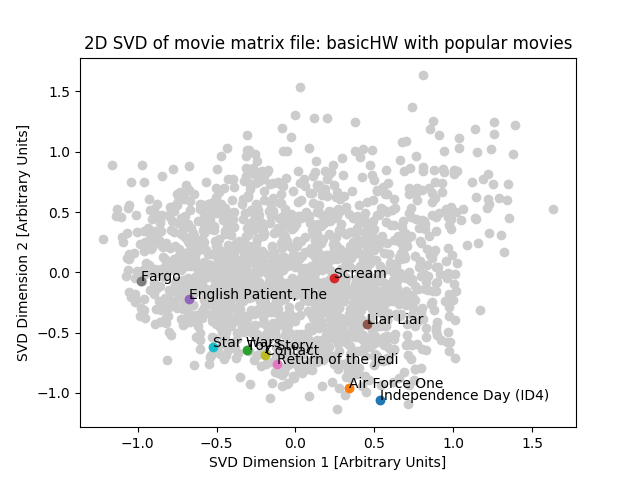
\includegraphics[width=0.75\textwidth]{../Figures/fig2.png}
    \caption{Ten most popular movies, using basic factorization from HW5.}
    \end{figure}

\subsection{The ten best movies}    
    \begin{figure}[H]
    \centering
    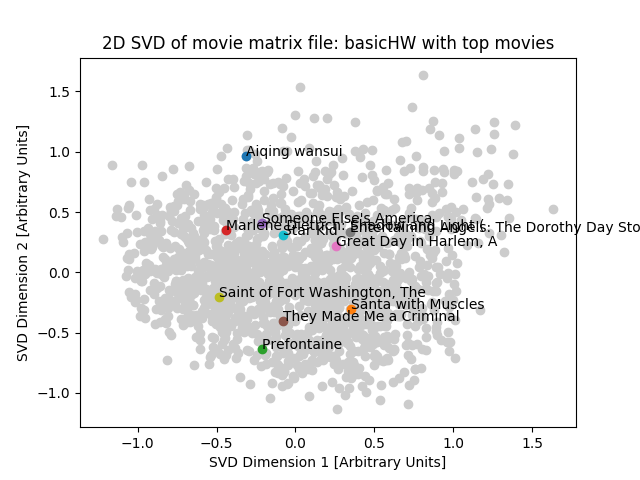
\includegraphics[width=0.75\textwidth]{../Figures/fig3.png}
    \caption{Ten best movies, using basic factorization from HW5.}
    \end{figure}

\subsection{Ten movies from the three genres selected in Section 4}
    \begin{figure}[H]
    \centering
    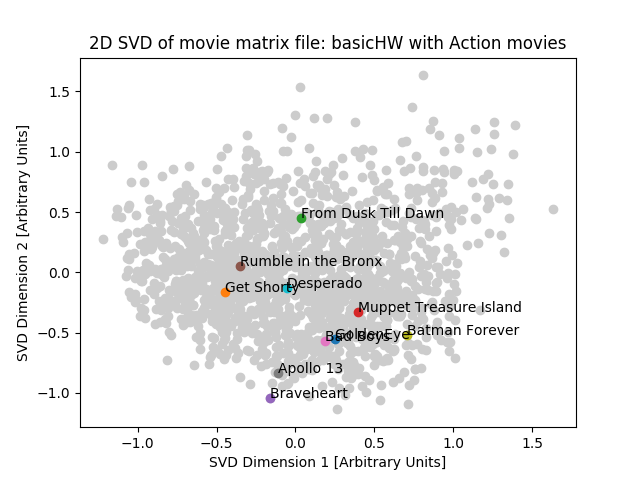
\includegraphics[width=0.6\textwidth]{../Figures/fig4a.png}
    \caption{Ten action movies, using basic factorization from HW5.}
    \end{figure}
    \begin{figure}[H]
    \centering
    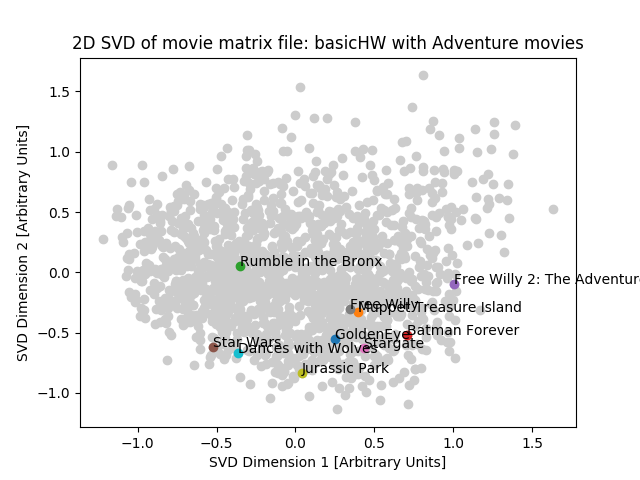
\includegraphics[width=0.6\textwidth]{../Figures/fig4b.png}
    \caption{Ten adventure movies, using basic factorization from HW5.}
    \end{figure}
    \begin{figure}[H]
    \centering
    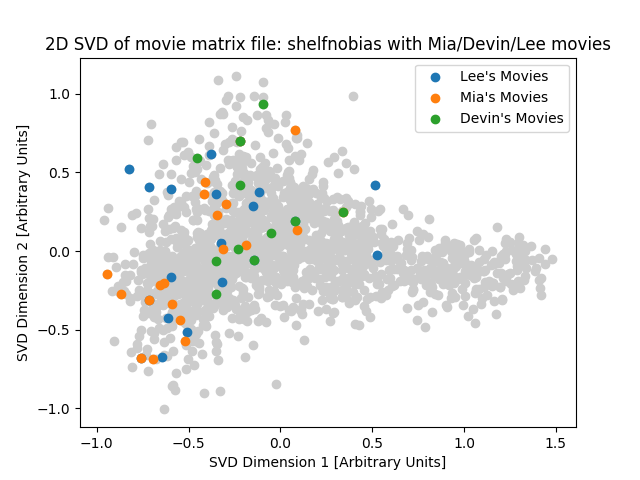
\includegraphics[width=0.6\textwidth]{../Figures/fig4c.png}
    \caption{Ten comedy movies, using basic factorization from HW5.}
    \end{figure}
    
    %\begin{figure}[H]
    %\centering
    %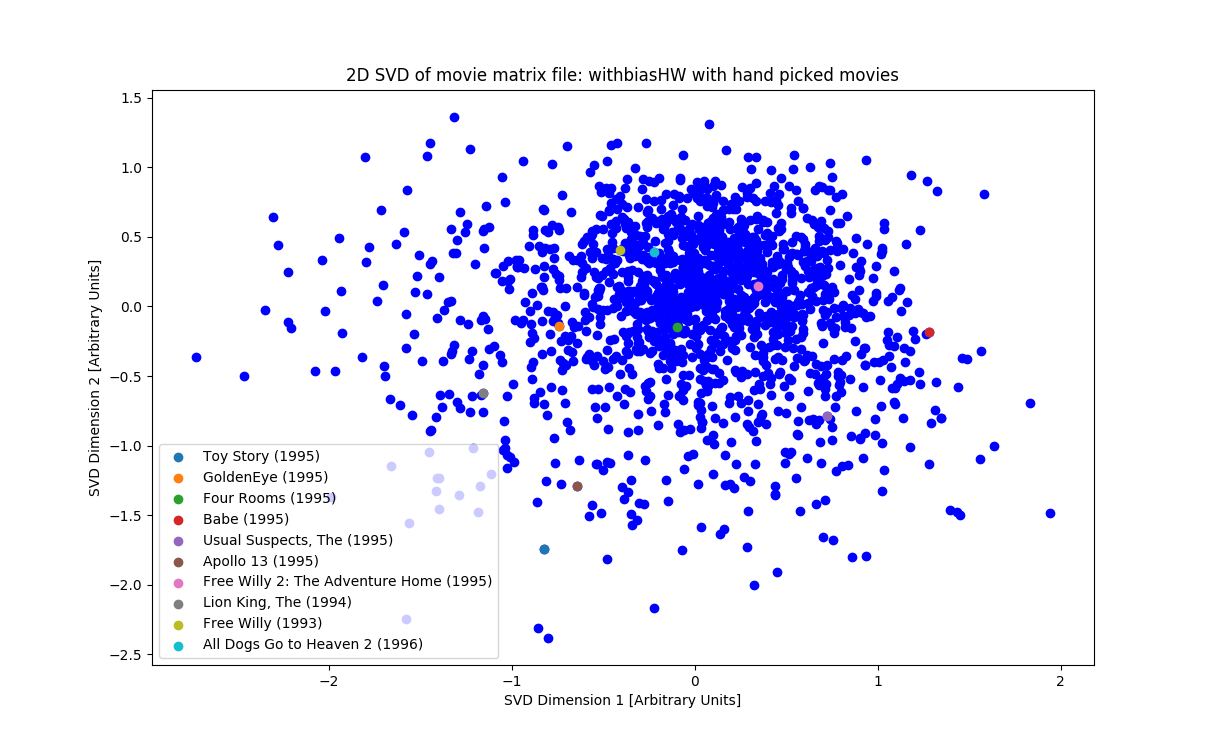
\includegraphics[width=0.75\textwidth]{../Figures/TenHandPickedMoviesBasicwBias.png}
    %\caption{Ten handpicked movies, basic, with bias.}
    %\end{figure}

    %\begin{figure}[H]
    %\centering
    %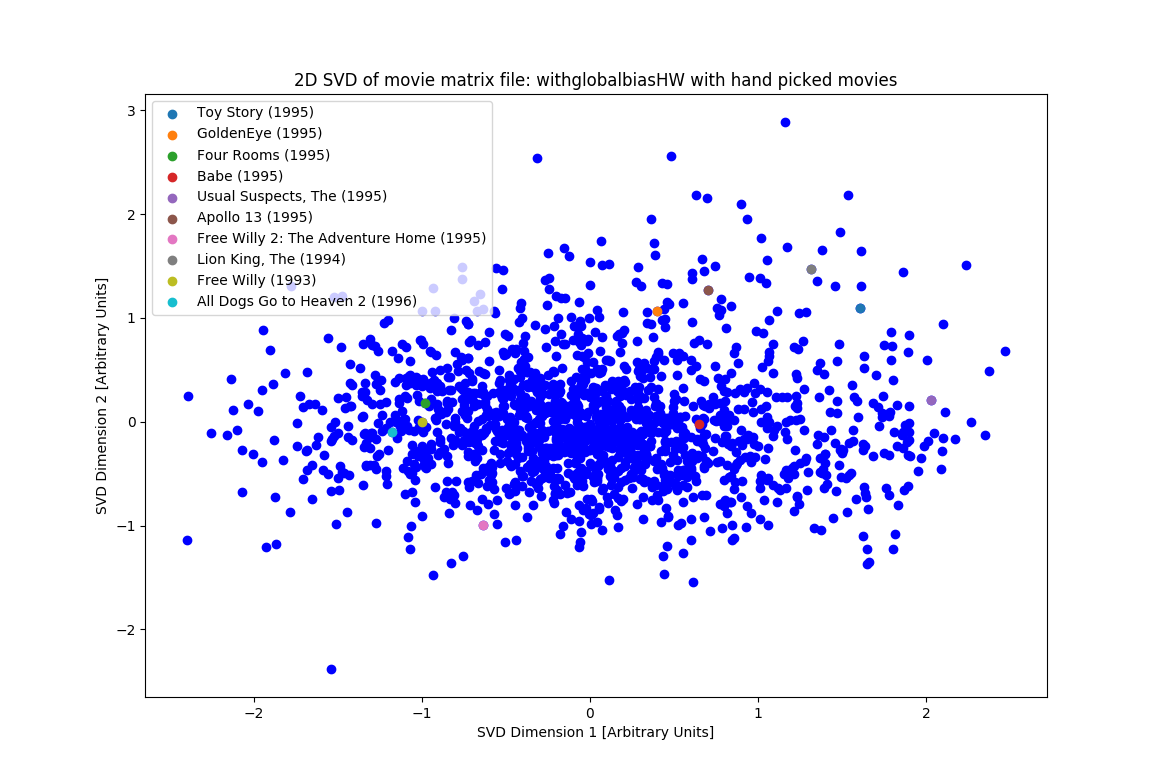
\includegraphics[width=0.75\textwidth]{../Figures/TenHandPickedMoviesBasicwGlobalBias.png}
    %\caption{Ten handpicked movies, basic, with global bias.}
    %\end{figure}


\end{document}
